\documentclass{article}

\usepackage{geometry}
\usepackage[super]{nth}
\usepackage{graphicx}

\title{Memory management basics with MOSS Memory Management Simulator -- an EOPSY laboratory}
\author{Maciej Marcinkiewicz}
\date{\nth{18} May 2021}

\newgeometry{lmargin=3.2cm, rmargin=3.2cm, bmargin=2.5cm}

\begin{document}

\maketitle

\section{Introduction}
\subsection{Brief description of the task}
The goal of this laboratory was to introduce students to the principles of memory management
in operating systems. As last time, a MOSS simulator came in handy for that purpose (Memory Management simulator to be more precise).
Laboratory's main task was to map any 8 pages of physical memory to the first 8 pages of virtual memory and then run simulation
to read each of 64 virtual memory pages.

\subsection{Environment description and configuration}
Simulator was configured in \texttt{memory.conf} file. Simulation environment consists of 64 virtual pages and 32 physical pages. Page size was defined as 16384 B.
Pages were mapped in the following way:

\noindent
\ttfamily
memset 0 0 0 0 0 0\\
memset 1 1 0 0 0 0      \\
memset 2 10 0 0 0 0      \\
memset 3 11 0 0 0 0      \\
memset 4 21 0 0 0 0      \\
memset 5 22 0 0 0 0      \\
memset 6 30 0 0 0 0      \\
memset 7 31 0 0 0 0
\rmfamily
.

The only columns that matter in these \texttt{memset} commands are the first and the second --
the first is a number of virtual page and the latter is the number of physical page mapped to
that virtual page.

The last part of setup was \texttt{commands} file. It describes the way simultion should work,
e.g. writing and reading data to/from specific memory addresses. For this laboratory it was set up
to read one virtual memory address from each of 64 virtual pages. Here is a sample of that file:

\noindent
\ttfamily
READ hex 0\\
READ hex 4000\\
READ hex 8000\\
READ hex C000\\
READ hex 10000\\
READ hex 14000\\
READ hex 18000\\
READ hex 1C000\\
READ hex 20000
\rmfamily
.

As page size was set to 16384 B, in order to read one address of each page simulation had
to read a one memory cell every  16384 B. As it is 4000$_{16}$ B, starting from 0x0 next addresses
are 0x4000, 0x8000, 0xC000, etc.

\section{Simulation results}
\subsection{Simulation output (tracefile)}
\ttfamily
\small
READ 0 ... okay\\
READ 4000 ... okay\\
READ 8000 ... okay\\
READ c000 ... okay\\
READ 10000 ... okay\\
READ 14000 ... okay\\
READ 18000 ... okay\\
READ 1c000 ... okay\\
READ 20000 ... okay\\
READ 24000 ... okay\\
READ 28000 ... okay\\
READ 2c000 ... okay\\
READ 30000 ... okay\\
READ 34000 ... okay\\
READ 38000 ... okay\\
READ 3c000 ... okay\\
READ 40000 ... okay\\
READ 44000 ... okay\\
READ 48000 ... okay\\
READ 4c000 ... okay\\
READ 50000 ... okay\\
READ 54000 ... okay\\
READ 58000 ... okay\\
READ 5c000 ... okay\\
READ 60000 ... okay\\
READ 64000 ... okay\\
READ 68000 ... okay\\
READ 6c000 ... okay\\
READ 70000 ... okay\\
READ 74000 ... okay\\
READ 78000 ... okay\\
READ 7c000 ... okay\\
READ 80000 ... page fault\\
READ 84000 ... page fault\\
READ 88000 ... page fault\\
READ 8c000 ... page fault\\
READ 90000 ... page fault\\
READ 94000 ... page fault\\
READ 98000 ... page fault\\
READ 9c000 ... page fault\\
READ a0000 ... page fault\\
READ a4000 ... page fault\\
READ a8000 ... page fault\\
READ ac000 ... page fault\\
READ b0000 ... page fault\\
READ b4000 ... page fault\\
READ b8000 ... page fault\\
READ bc000 ... page fault\\
READ c0000 ... page fault\\
READ c4000 ... page fault\\
READ c8000 ... page fault\\
READ cc000 ... page fault\\
READ d0000 ... page fault\\
READ d4000 ... page fault\\
READ d8000 ... page fault\\
READ dc000 ... page fault\\
READ e0000 ... page fault\\
READ e4000 ... page fault\\
READ e8000 ... page fault\\
READ ec000 ... page fault\\
READ f0000 ... page fault\\
READ f4000 ... page fault\\
READ f8000 ... page fault\\
READ fc000 ... page fault

\rmfamily
\normalsize

\subsection{Comments}
\begin{figure}[h!]
    \centering
        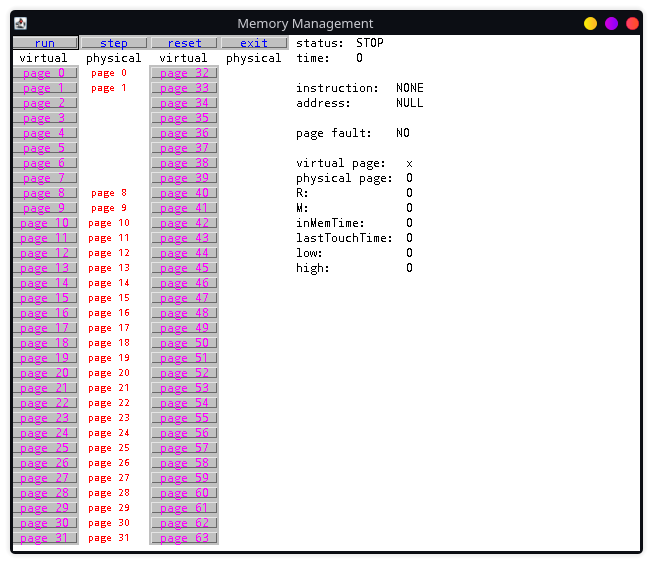
\includegraphics[width=0.7\linewidth]{img/initial_state.png}
    \caption{Initial state of simulation.}
\end{figure}

In the beginning physical pages 0-31 are assigned to virtual pages 0-31 (fig. 1). Pages 
8-31 are mapped by simulator (probably it is its default behaviour). Due
to some sort of glitch simulator does not show changes that had been made to virtual pages
2-7, however inspecting each of these virtual pages show that they are indeed mapped with
those physical pages mentioned in the introduction to this laboratory.

Before running the simulation it is clear that starting from page 32 up to the final one
it will encounter \emph{page faults}. Page fault happens when a non-mapped virtual page
is being referenced. In such case a \emph{page replacement} algorithm should work and
map a physical page by itself. The first requested address with page fault would be
0x80000 -- 32 pages were mapped, so it had to be \nth{33} page and $32_{10} \cdot 4000_{16} = 80000_{16}$.

Tracefile produced by simulator shows that in fact page 32 is the first one which encountered
a page fault. Fig. 2 shows that the replacement order of pages is the same as pages mapping
for the first half of virtual pages. For instance, virtual page 36 had been mapped to physical
page 21, so the same page as it was mapped to page 4.
\newpage
\begin{figure}[h!]
    \centering
        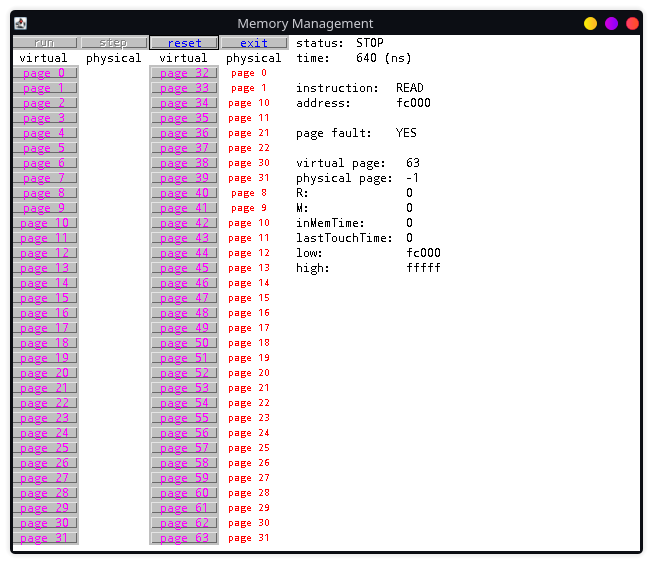
\includegraphics[width=0.7\linewidth]{img/final_state.png}
    \caption{Final state of simulation.}
\end{figure}

Such behaviour means that the page replacement algorithm has to be \emph{First In, First Out} (FIFO).
Operating system is tracking every page in queue, so when there is a need for page replacement,
it uses page from the front of the queue, i.e. the oldest page.

\end{document}